%//==============================--@--===========================//%
\clearpage
\subsection[5.4 MAC addressing and ARP protocol]{\hspace*{0.075 em}\raisebox{0.2 em}{$\pmb{\drsh}$} MAC addressing and ARP protocol}
\label{subsec:MAC}

\noindent A link-layer address is variously called a LAN address, a physical address, or a MAC address.

\begin{itemize}
    \item The MAC address is 6 bytes long, giving $2^{48}$ possible MAC addresses. 
    \item The Mac address is expressed in hexadecimal notation.
    \item  MAC addresses were designed to be permanent (however there exists software which allows one to alter them).
    \item IEEE manages the MAC address space. 
    \item Each adapter has it's own unique MAC address.
    \item An adapter’s MAC address has a flat structure (as opposed to a hierarchical structure) and doesn’t change no matter where the adapter goes.
    \item When an adapter receives a frame, it will check to see whether the destination MAC address in the frame matches its own MAC address. If there is a match, the adapter extracts the enclosed datagram and passes the datagram up the protocol stack, if not, the adapter discards the frame.
\end{itemize}

\vspace{1 em}
\noindent\textbf{Nota:}
An adapter may choose to broadcast it's frame to all available adapters in the LAN. To do so it uses a \textbf{MAC brodcast address}: \texttt{FF-FF-FF-FF-FF-FF}.

\vspace{-1em}
\begin{figure}[H]
    \centering
    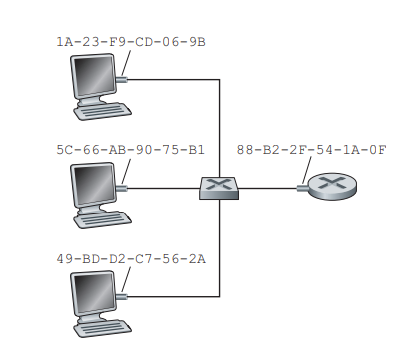
\includegraphics[width = 0.6\linewidth]{img/5/MAC-address-example.png}
    \caption{Each interface connected to a LAN has a unique MAC address. Notice that the switch does not possess a MAC address in each of their interfaces, this is because the job of the link-layer switch is to carry datagrams between hosts and routers; a switch does this job transparently, that is, without the host or router having to explicitly address the frame to the intervening switch}
    \label{fig:MAC-address-example}
\end{figure}

\begin{mdframed}
    \textbf{MAC address spoofing} is a technique where an attacker manipulates the unique hardware identifier (Media Access Control address) of a network interface, allowing them to impersonate other devices, bypass access controls, or evade monitoring on a network.
\end{mdframed}

%//==============================--@--==============================//%
\clearpage
\subsubsection[5.4.1 Address Resolution Protocol (ARP)]{$\rightarrow$ Address Resolution Protocol (ARP)}

\noindent An ARP module in the sending host takes any IP address on the same LAN as input, and returns the corresponding MAC address of the destination. Each host and router has an \textbf{ARP table} in its memory, which contains mappings of IP addresses to MAC addresses. It also contains a time-to-live (TTL) value, which indicates when each mapping will be deleted from the table.

\begin{figure}[H]
    \centering
    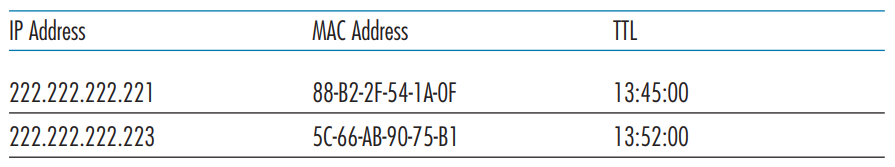
\includegraphics[width = 0.75\linewidth]{img/5/ARP-table.png}
    \caption{Example of an ARP table \cite{Kurose2017}}
    \label{fig:ARP-table}
\end{figure}

\noindent\textbf{Note:} ARP resolves IP addresses for \underline{hosts and router interfaces} \textbf{on the same subnet}.

\vspace{1 em}
\noindent The ARP protocol is defined by the following steps:

\begin{enumerate}
    \item The sending host checks if the ARP table contains an entry for the destination node's IP address.
    \item If not, the sender constructs an ARP query packet containing the sending and receiving IP and MAC addresses.
    \item The sender passes the ARP query packet to the adapter, indicating to send the packet to the MAC broadcast address (\texttt{FF-FF-FF-FF-FF-FF}).
    \item The adapter encapsulates the ARP packet in a link-layer frame and transmits it into the subnet using the broadcast address.
    \item All adapters on the subnet receive the frame and pass the ARP packet to their ARP modules.
    \item The ARP modules check if their IP address matches the destination IP address in the ARP packet.
    \item The module with a matching IP address sends a response ARP packet back to the querying host with the desired IP-to-MAC mapping.
    \item The querying host updates its ARP table and sends its IP datagram, encapsulated in a link-layer frame with the destination MAC obtained from the ARP response.
\end{enumerate}

\begin{figure}[H]
    \centering
    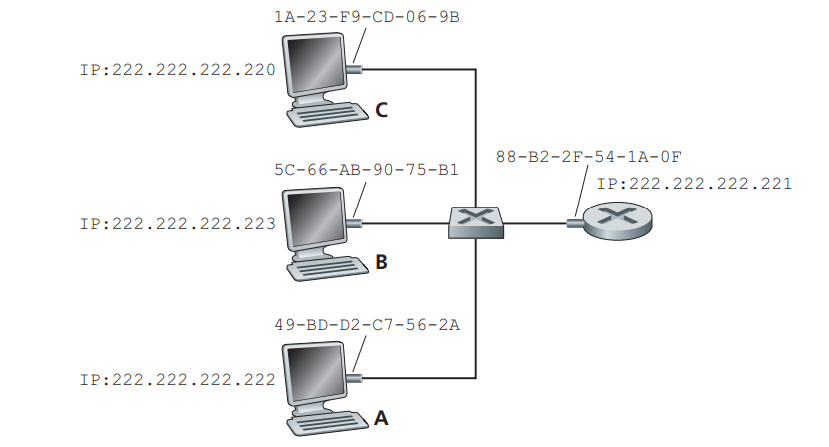
\includegraphics[width = 0.7\linewidth]{img/5/MAC-IP-LAN.png}
    \caption{Each interface on a LAN has an IP address and a MAC address \cite{Kurose2017}}
    \label{fig:MAC-IP-LAN}
\end{figure}

%//==============================--@--===========================//%
\clearpage
\paragraph[5.4.1 Sending a Datagram off the Subnet]{$\pmb{\star}$ Sending a Datagram off the Subnet}\mbox{}\\[4pt]
\noindent Sending a datagram off the subnet is more complicated than sending it within the subnet. Let's consider a network with two subnets interconnected by a router. In this scenario, each host has one IP address and one adapter, while a router has an IP address for each of its interfaces, as well as an ARP module and an adapter for each interface.

\begin{figure}[H]
    \centering
    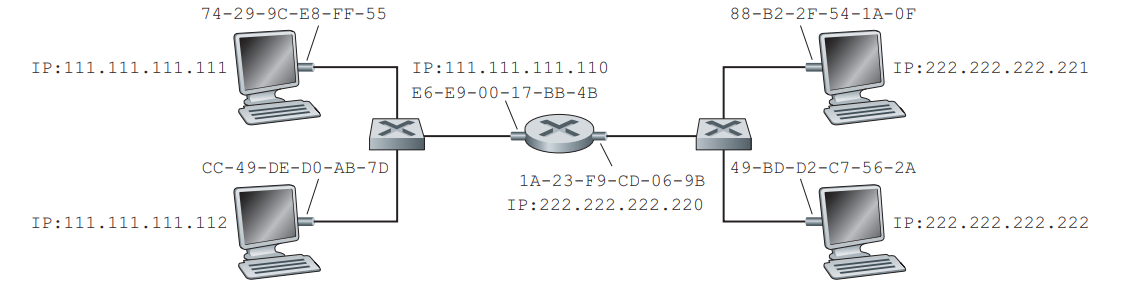
\includegraphics[width = 1\linewidth]{img/5/sending-datagram-two-subnets.png}
    \caption{Two subnets interconnected by a router \cite{Kurose2017}}
    \label{fig:sending-datagram-two-subnets}
\end{figure}

\noindent Assume that host A wants to send an IP datagram to host B on a different subnet. The sender must pass the datagram to its adapter and indicate an appropriate destination MAC address. But, using the MAC address of the adapter for host B directly would be incorrect, as the datagram would not pass through any adapters on the sender's subnet\footnotemark[6].

Instead, the appropriate MAC address for the frame should be that of the router interface on the sender's subnet, which can be obtained using ARP. After creating a frame containing the datagram addressed to host B, the sender sends it to the router interface on its subnet. The router then forwards the datagram to the router interface on the destination subnet, which sends the frame into that subnet. Finally, the destination MAC address of the frame is indeed the MAC address of the ultimate destination (host B), which is also obtained via ARP.

\vspace{1 em}
\noindent The general behavior of sending datagrams off of a subnet to another can be summarized as follows:
\begin{enumerate}
    \item The sender checks the destination IP address and uses ARP to obtain the MAC address of the router interface on its subnet, if needed.
    \item The sender creates a frame containing the datagram addressed to the destination host, using the MAC address obtained in the previous step.
    \item The sender's adapter transmits the frame onto its subnet; the router's adapter on the sender's subnet receives it and passes the datagram to the router's network layer.
    \item The router consults its forwarding table, determines the correct output interface, and uses ARP to obtain the destination MAC address for the destination host or next-hop router interface.
    \item The router's adapter on the destination subnet encapsulates the datagram in a new frame with the obtained MAC address and transmits it onto the destination subnet.
    \item The destination host's adapter receives the frame and passes the datagram to its network layer.
\end{enumerate}

\footnotetext[6]{``The datagram would just die and go to datagram heaven.''\protect\cite{Kurose2017}}

%//==============================--@--===========================//%
\clearpage 
\subsubsection[5.4.2 Ethernet]{$\rightarrow$ Ethernet}

\noindent Ethernet is a widely used local area network (LAN) technology that provides a communication protocol for transmitting data packets over wired connections.

\vspace{1em}
\noindent Ethernet has dominated the wired LAN market since the 1970s due to its early deployment, simplicity, cost-effectiveness, and continuous evolution in data rates. Initially using a coaxial bus topology, Ethernet transitioned to a hub-based star topology in the late 1990s, which still operated as a broadcast LAN. In the early 2000s, the hub was replaced with a switch, making Ethernet collision-less and transforming it into a store-and-forward packet switch that operates up to layer 2. This evolution has contributed to Ethernet's ongoing success and prevalence in local area networking.

\begin{figure}[H]
    \centering
    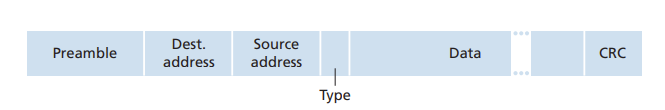
\includegraphics[width = 1\linewidth]{img/5/Ethernet.png}
    \caption{Ethernet frame structure \cite{Kurose2017}}
    \label{fig:ethernet}
\end{figure}

\begin{itemize}
\item \textbf{Preamble} (8 bytes): serves to "wake up" the receiving adapters and synchronize their clocks to that of the sender's clock. The first 7 bytes have a value of 10101010, and the last byte is 10101011. The last two bits of the 8th byte alert the receiving adapter that the "important stuff" is about to come.

\item \textbf{Destination address} (6 bytes): contains the MAC address of the destination adapter.

\item \textbf{Source address} (6 bytes): contains the MAC address of the sending adapter.

\item \textbf{Type field} (2 bytes): allows Ethernet to multiplex network-layer protocols, such as IP, Novell IPX, AppleTalk, and ARP, among others. Each protocol has its own standardized type number.

\item \textbf{Data field} (46 to 1,500 bytes): carries the IP datagram, requires padding or fragmentation as needed. The maximum transmission unit (MTU) of Ethernet is 1,500 bytes. If the IP datagram exceeds 1,500 bytes, the host has to fragment the datagram. If the IP datagram is less than 46 bytes, the data field has to be "stuffed" to fill it out to 46 bytes.

\item \textbf{Cyclic redundancy check (CRC)} (4 bytes): allows the receiving adapter to detect bit errors in the frame. The receiving adapter runs a CRC check but does not send an acknowledgment for passed frames nor a negative acknowledgment for failed frames.
\end{itemize}

\noindent Ethernet technologies provide an unreliable and connectionless service at the link layer, analogous to IP's layer-3 datagram service and UDP's layer-4 connectionless service. Ethernet has evolved into different flavors, such as
\begin{itemize}[nolistsep,noitemsep,label=--]\small
    \item \texttt{10BASE-T}: 10 Mbps over twisted-pair copper cables
    \item \texttt{10BASE-2}: 10 Mbps over thin coaxial cables
    \item \texttt{100BASE-T}: 100 Mbps over twisted-pair copper cables
    \item \texttt{1000BASE-LX}: 1 Gbps over long-wavelength single-mode fiber-optic cables
    \item \texttt{10GBASE-T}: 10 Gbps over twisted-pair copper cables
    \item \texttt{40GBASE-T}: 40 Gbps over twisted-pair copper cables
\end{itemize}
standardized by the IEEE 802.3 CSMA/CD (Ethernet) working group.

%//==============================--@--===========================//%